\RequirePackage{plautopatch}
\documentclass[uplatex,dvipdfmx,a4paper,11pt]{jlreq}
\usepackage{bxpapersize}
\usepackage[utf8]{inputenc}
\usepackage{fontenc}
\usepackage{lmodern}
\usepackage{otf}
\usepackage{amsmath}
\usepackage{amssymb}
\usepackage{amsthm}
\usepackage{ascmac}
% \usepackage[hyphens]{url}
\usepackage{mhchem}
\usepackage{siunitx}
\usepackage{physics2}
\usephysicsmodule{ab, ab.braket, doubleprod, diagmat, xmat}
\usepackage[DIF = {
op-symbol = d,
op-order-nudge = 1 mu,
outer-Ldelim = \left . ,
outer-Rdelim = \right |,
sub-nudge = 0 mu
}]{diffcoeff}
% \usepackage{braket}
\usepackage{verbatimbox}
\usepackage{bm}
\usepackage{url}
% \usepackage[dvipdfmx,hiresbb,final]{graphicx}
\usepackage{hyperref}
\usepackage{pxjahyper}
\usepackage{tikz}\usetikzlibrary{cd}
\usepackage{tikz-feynhand}
\usepackage{listings}
\usepackage{color}
\usepackage{mathtools}
\usepackage{xspace}
\usepackage{xy}
\usepackage{xypic}
%
\title{原子核物理学}
\author{anko9801}
\makeatletter
%
\DeclareMathOperator{\lcm}{lcm}
\DeclareMathOperator{\Kernel}{Ker}
\DeclareMathOperator{\Image}{Im}
\DeclareMathOperator{\ch}{ch}
\DeclareMathOperator{\Aut}{Aut}
\DeclareMathOperator{\Log}{Log}
\DeclareMathOperator{\Arg}{Arg}
\DeclareMathOperator{\sgn}{sgn}
%
\newcommand{\CC}{\mathbb{C}}
\newcommand{\RR}{\mathbb{R}}
\newcommand{\QQ}{\mathbb{Q}}
\newcommand{\ZZ}{\mathbb{Z}}
\newcommand{\NN}{\mathbb{N}}
\newcommand{\FF}{\mathbb{F}}
\newcommand{\PP}{\mathbb{P}}
\newcommand{\GG}{\mathbb{G}}
\newcommand{\TT}{\mathbb{T}}
\newcommand{\EE}{\bm{E}}
\newcommand{\BB}{\bm{B}}
\renewcommand{\AA}{\bm{A}}
\newcommand{\rr}{\bm{r}}
\newcommand{\kk}{\bm{k}}
\newcommand{\pp}{\bm{p}}
\newcommand{\calB}{\mathcal{B}}
\newcommand{\calF}{\mathcal{F}}
\newcommand{\ignore}[1]{}
\newcommand{\floor}[1]{\left\lfloor #1 \right\rfloor}
% \newcommand{\abs}[1]{\left\lvert #1 \right\rvert}
\newcommand{\lt}{<}
\newcommand{\gt}{>}
\newcommand{\id}{\mathrm{id}}
\newcommand{\rot}{\curl}
\renewcommand{\angle}[1]{\left\langle #1 \right\rangle}
\newcommand{\lbar}{\lambda \kern -0.5em\raise 0.5ex \hbox{--}}
\newcommand\mqty[1]{\begin{pmatrix}#1\end{pmatrix}}
\newcommand\vmqty[1]{\begin{vmatrix}#1\end{vmatrix}}
\numberwithin{equation}{section}

\let\oldcite=\cite
\renewcommand\cite[1]{\hyperlink{#1}{\oldcite{#1}}}

\let\oldbibitem=\bibitem
\renewcommand{\bibitem}[2][]{\label{#2}\oldbibitem[#1]{#2}}

% theorem環境の設定
% - 冒頭に改行
% - 末尾にdiamond (amsthm)
\theoremstyle{definition}
\newcommand*{\newscreentheoremx}[2]{
  \newenvironment{#1}[1][]{
    \begin{screen}
    \begin{#2}[##1]
      \leavevmode
      \newline
  }{
    \end{#2}
    \end{screen}
  }
}
\newcommand*{\newqedtheoremx}[2]{
  \newenvironment{#1}[1][]{
    \begin{#2}[##1]
      \leavevmode
      \newline
      \renewcommand{\qedsymbol}{\(\diamond\)}
      \pushQED{\qed}
  }{
      \qedhere
      \popQED
    \end{#2}
  }
}
\newtheorem{theorem*}{定理}[section]

\newqedtheoremx{theorem}{theorem*}
\newcommand*\newqedtheorem@unstarred[2]{%
  \newtheorem{#1*}[theorem*]{#2}
  \newqedtheoremx{#1}{#1*}
}
\newcommand*\newqedtheorem@starred[2]{%
  \newtheorem*{#1*}{#2}
  \newqedtheoremx{#1}{#1*}
}
\newcommand*{\newqedtheorem}{\@ifstar{\newqedtheorem@starred}{\newqedtheorem@unstarred}}

\newtheorem{sctheorem*}{定理}[section]
\newscreentheoremx{sctheorem}{sctheorem*}
\newcommand*\newscreentheorem@unstarred[2]{%
  \newtheorem{#1*}[theorem*]{#2}
  \newscreentheoremx{#1}{#1*}
}
\newcommand*\newscreentheorem@starred[2]{%
  \newtheorem*{#1*}{#2}
  \newscreentheoremx{#1}{#1*}
}
\newcommand*{\newscreentheorem}{\@ifstar{\newscreentheorem@starred}{\newscreentheorem@unstarred}}

%\newtheorem*{definition}{定義}
%\newtheorem{theorem}{定理}
%\newtheorem{proposition}[theorem]{命題}
%\newtheorem{lemma}[theorem]{補題}
%\newtheorem{corollary}[theorem]{系}

\newqedtheorem{lemma}{補題}
\newqedtheorem{corollary}{系}
\newqedtheorem{example}{例}
\newqedtheorem{proposition}{命題}
\newqedtheorem{remark}{注意}
\newqedtheorem{thesis}{主張}
\newqedtheorem{notation}{記法}
\newqedtheorem{problem}{問題}
\newqedtheorem{algorithm}{アルゴリズム}

\newscreentheorem*{axiom}{公理}
\newscreentheorem*{definition}{定義}

\renewenvironment{proof}[1][\proofname]{\par
  \normalfont
  \topsep6\p@\@plus6\p@ \trivlist
  \item[\hskip\labelsep{\bfseries #1}\@addpunct{\bfseries}]\ignorespaces\quad\par
}{%
  \qed\endtrivlist\@endpefalse
}
\renewcommand\proofname{証明}

\makeatother

\begin{document}
\maketitle
\tableofcontents
\clearpage

\section{原子核}
物質はすべて分子や原子によって構成されている。
例えば水は \ce{H2O} の分子で出来ており水素原子と酸素原子が結合してできている。
その原子は原子核と電子で構成されており、原子核は陽子と中性子によって構成されている。
この陽子と中性子を核子と呼び、核子は核力を受けながら原子核中を飛び回っている。

その核力を解明し、核反応によって陽子と中性子が互いに遷移し合うような現象や原子核に関する魔法数、ビッグバン時や星の一生でどのように原子核が構成されるかなど、これらすべてを説明するようなモデルを構築することこそが原子核物理学である。

実験結果、描像、原子核を構成、原子核の性質

\subsection{原子核の発見}
1897 年: 電子の発見 J.J. Thomson, 陰極線の実験

1904 年: Plum pudding model (ブドウパンモデル) J.J. Thomson が提唱

1904 年: 土星型原子モデル 長岡半太郎が提唱

1909 年: ラザフォード (Rutherford) の散乱実験により原子核の大きさ
アーネスト・ラザフォードの弟子のハンス・ガイガーとアーネスト・マースデンによる実験
$\alpha$ 線を金箔に照射し、2万回に1回ほど90度以上の角度に散乱

1956 年: ホフスタッター (Robert Hofstadter) の電子散乱実験により原子核の形状が分かった。

電荷 $Ze$
フェルミ粒子で構成→スピン半整数
窒素分子の回転バンドやラマン分光の測定→スピン整数

James Chadwick による中性子の発見
\begin{align}
  \ce{^4_2He} + \ce{^9_4Be_5} \to \ce{^12_6C_6} + n
\end{align}
未知の中性粒子によって弾かれた陽子を検出器で観測
中性粒子の質量が陽子と同程度であることを見いだした
(γ線だと仮定すると極めて高いエネルギーになる)


\subsection{散乱理論}
\begin{align}
  \diff{\sigma}{\Omega} = \ab(\frac{a}{4E})^{\frac{1}{2}}\sin4(\theta/2)
\end{align}
\begin{align}
  d_0                   & = \frac{a}{E} = \frac{\alpha z Z(\hbar c)}{E} \\
  \dl{N}                & = 2\pi b\dl{l}N                               \\
  b                     & = \frac{a}{2E}\cot\frac{\theta}{2}            \\
  \dl{\sigma}           & = \frac{\dl{N}}{N}                            \\
  \diff{\sigma}{\Omega} & = \frac{1}{N}\diff{N}{\Omega} =
\end{align}
https://www.nobelprize.org/prizes/physics/1961/hofstadter/lecture/

\subsection{核子}
陽子と中性子はどちらもスピン 1/2 のフェルミオンである。
\begin{align}
  m_p & = 938.272\ \si{MeV/c^2} \\
  m_n & = 939.565\ \si{MeV/c^2} \\
  m_e & = 0.511\ \si{MeV/c^2}
\end{align}
核子は水素原子の電子と同じような軌道となるのか?

原子核の半径 $R$ は核子 1 個当たりの半径 $r_0 = 1.25$ \si{fm} から求まる。
\begin{align}
  R = r_0A^{1/3}
\end{align}
体積が質量数 $A$ に比例することから密度の飽和性がわかる。
\begin{align}
  \ab<r^2> & = \int r^2\rho(\rr)\dl[3]{r} = \int r^2\rho(\rr)4\pi r^2\dl{r}
  \frac{5}{3}
\end{align}

原子核の形状はさまざまな近似方法があるが最も広く使われている Woods-Saxon 型分布 (Fermi 関数) という原子核の形状因子を紹介する。
標準核密度 $\rho_0 = 0.17$ \si{fm^{-3}} diffuseness $a \approx 0.67$ \si{fm} を用いて
\begin{align}
  \rho(r) & = \frac{\rho_0}{1 + \exp\ab(-\dfrac{r - R}{a})}
\end{align}
これは次のようなグラフとなる。
平均核子間距離 $d = \langle\rho\rangle^{-1/3}$



\subsection{フェルミガス模型}
まずは核子間で相互作用することなく自由に運動しているモデルを考える。 \\

1 辺 $L$ の立方体の中に $N$ 個の中性子を入れる。
\begin{align}
  \bm{k}    & = \ab(\frac{2\pi}{L}n_x, \frac{2\pi}{L}n_y, \frac{2\pi}{L}n_z)                                                                       \\
  \psi(\rr) & = e^{i\kk\cdot\rr}                                                                                                                   \\
  dn        & = 4\pi k^2dk \times 2 \ab(\frac{2\pi}{L})^3 = \frac{V}{\pi^2}k^2dk                                                                   \\
  N         & = \int_0^{k_F}\diff{n}{k}\dl{k} = \frac{V}{3\pi^2}k_F^3                                                                              \\
  k_F       & = \ab(\frac{3\pi^2 N}{V})^{1/3}                                                                                                      \\
  E_F       & = \frac{p_F^2}{2m} = \frac{(\hbar k_F)^2}{2m} = \frac{\hbar^2}{2m}\ab(\frac{3\pi^2 N}{V})^{2/3}                                      \\
  n         & = 2\int d\rr \int d\pp \frac{1}{h^3} = 2\frac{\Omega}{(2\pi)^3}\int_0^{k_F}4\pi k^2dk = 2\frac{\Omega}{(2\pi)^3}\frac{4}{3}\pi k_F^3 \\
  k_F       & = \ab(3\pi^2\frac{n}{\Omega})^{1/3}
\end{align}
\begin{align}
  P_{Fn} & = \hbar k_{Fn} = \hbar\ab(3\pi^2\rho_n)^{1/3} \\
  P_{Fp} & = \hbar k_{Fp} = \hbar\ab(3\pi^2\rho_p)^{1/3}
\end{align}

フェルミガス模型に従うことから核子が原子核中でかなり自由に動いていることがわかる。
からスピン 1/2 と -1/2 の 2 つがあり、異なるスピンとしか衝突しない。
実際光速の 20 \% 程度で移動している。
陽子や中性子の平均自由行程が長くなる。
統計力学



\subsection{独立粒子模型}
多数の実験結果から陽子または中性子の数が 2, 8, 20, 28, 50, 82, 126 のとき結合エネルギーが大きく、安定していることが結論づけられている。
これを魔法数 (magic number) と呼ぶ。

原子核は核子の多体問題となっているが、フェルミガス模型から分かるように核子同士の相互作用を無視する独立粒子模型がよい近似となっていることがわかる。
これより他の核子からの核力の平均の場中で核子の運動を考える平均場近似をする。
その平均場でよく用いられる Woods-Saxon Potential は次のようになる。
\begin{align}
  V(r) & = -\frac{U_0}{1 + \exp\ab(\dfrac{r - R}{a})}
\end{align}
Woods-Saxon Potential はシュレーディンガー方程式で解析的に解けないので調和振動子のポテンシャルに近似する。
\begin{align}
  V(r) & = -V_0 + \frac{1}{2}m\omega^2r^2 \qquad (V_0 = 40\ \si{MeV})
\end{align}
このとき量子力学でやったように 3 次元極座標系の微分方程式を解くと波動関数 $\psi_{nlm}(\rr) = R_{nl}(r)Y_{lm}(\theta, \varphi)$ に対してエネルギーは次のようになる。
\begin{align}
  H & = -\frac{\hbar^2}{2m}\nabla^2 + \frac{1}{2}m\omega^2r^2 \\
  E & = \ab(2n + l + \frac{3}{2})\hbar\omega
\end{align}
これより $N = 2n + l$ とおくと表 \ref{table:oscillator} のようになる。
\begin{table}[hbtp]
  \centering
  \begin{tabular}{|c|c|c|c|c|c|c|}
    \hline
    表示 & $N$ & $n$ & $l$ & $m$                & 縮退度 & 殻     \\
    \hline \hline
    1s & 0   & 0   & 0   & 0                  & 2   & 1(2)  \\
    1p & 1   & 0   & 1   & $-1,0,1$           & 6   & 2(8)  \\
    1d & 2   & 0   & 2   & $-2,-1,0,1,2$      & 10  & 3(20) \\
    2s & 2   & 1   & 0   & 0                  & 2   & 3(20) \\
    1f & 3   & 0   & 3   & $-3,-2,-1,0,1,2,3$ & 14  & 4(40) \\
    2d & 3   & 1   & 1   & $-1,0,1$           & 6   & 4(40) \\
    \hline
  \end{tabular}
  \caption{調和振動子系の縮退度}
  \label{table:oscillator}
\end{table}
これより平均場近似では魔法数 2, 8, 20, 28, 50, 82, 126 を説明することはできない。

統計力学を考える。核子が埋まっている
\begin{align}
  D                       & = \sum_{N = 0}^{N_{\max}}(N + 1)(N + 2) = \frac{1}{3}(N_{\max} + 1)(N_{\max} + 2)(N_{\max} + 3)                         \\
  A                       & = 2D \approx \frac{2}{3}(N_{\max} + 2)^3                                                                                \\
  \bra<N|r^2\ket|N>       & = \bra<N|x^2 + y^2 + z^2\ket|N> = \frac{\hbar}{m\omega}\ab(N + \frac{3}{2})                                             \\
  A\ab<r^2>               & = \sum_{N = 0}^{N_{\max}}\frac{\hbar}{m\omega}\ab(N + \frac{3}{2})2(N + 1)(N + 2)                                       \\
                          & = \frac{1}{2}\frac{\hbar}{m\omega}(N_{\max} + 1)(N_{\max} + 2)^2(N_{\max} + 3)                                          \\
                          & \approx\frac{1}{2}\frac{\hbar}{m\omega}(N_{\max} + 2)^4 \approx \frac{1}{2}\frac{\hbar}{m\omega}\ab(\frac{3}{2}A)^{4/3} \\
  \ab<r^2>                & = \frac{\int_0^Rr^24\pi r^2\dl{r}}{\int_0^R4\pi r^2\dl{r}} = \frac{3}{5}R^2 = \frac{3}{5}r_0^2A^{2/3}                   \\
  \frac{3}{5}r_0^2A^{5/3} & \approx \frac{1}{2}\frac{\hbar}{m\omega}\ab(\frac{3}{2}A)^{4/3}                                                         \\
  \hbar\omega             & \approx \frac{5}{4}\ab(\frac{3}{2})^{1/3}\frac{\hbar^2}{mr_0^2}A^{-1/3} \approx 40A^{-1/3}\ \si{MeV}
\end{align}
結合エネルギーの飽和性 $V_0 \approx 50$ \si{MeV}

Mayer, Jensen はスピン軌道結合力 (L-S 力) を取り入れることで魔法数を説明した。
\begin{align}
  V(r) = -V_0 + \underbrace{\frac{1}{2}m\omega^2r^2}_{調和振動⼦} + \underbrace{V_{ls}\bm{l}\cdot\bm{s}}_{スピン軌道結合力}
\end{align}
\begin{align}
  \ab<\bm{l}\cdot\bm{s}> & = \frac{1}{2}[\bm{j}^2 - \bm{l}^2 - \bm{s}^2] = \frac{1}{2}\ab(j(j + 1) - l(l + 1) - s(s + 1)) \\
                         & = \frac{1}{2}\ab(j(j + 1) - l(l + 1) - \frac{3}{4})                                            \\
                         & = \begin{dcases}
                               \frac{1}{2}l         & (j = l + 1/2) \\
                               \frac{1}{2}(- l - 1) & (j = l - 1/2) \\
                             \end{dcases}
\end{align}
多数の実験結果から $V_{ls} = -20A^{-2/3}$ \si{MeV} となることが分かっている。
\begin{align}
  \Delta\varepsilon_{ls} & = V_{ls}\ab<\bm{l}\cdot\bm{s}> = \begin{dcases}
                                                              -10A^{-2/3}l       & (j = l + 1/2) \\
                                                              +10A^{-2/3}(l + 1) & (j = l - 1/2) \\
                                                            \end{dcases}
\end{align}
スピン軌道結合⼒よりスピンと軌道角運動量が同じ向きの方が安定する。
これが強い理由に軸性ベクトル (擬ベクトル) の話がある。
原子核の内部では力が働かず、表面において強い相互作用が働く P-inv, T-inv となるから
\begin{align}
  V(r) = -V_0 + \underbrace{\frac{1}{2}m\omega^2r^2}_{調和振動⼦} + \underbrace{V_{ls}\bm{l}\cdot\bm{s}}_{スピン軌道結合力} + \underbrace{D\bm{l}^2}_{表面項}
\end{align}



\subsection{核スピン}
各核子の波動関数は軌道 $(n, l, j^\pi)$ に依存する。spdfghi
\begin{table}[hbtp]
  \centering
  \begin{tabular}{|c|c|c|c|c|}
    \hline
    $(n, l, j^\pi)$ & 表示         & 縮退度 & パリティ & 核 (魔法数) \\
    \hline \hline
    $(0, 0, 1/2)$   & $1s_{1/2}$ & 2   & $+$  & 1 (2)   \\
    $(0, 1, 3/2)$   & $1p_{3/2}$ & 4   & $-$  & 2 (8)   \\
    $(0, 1, 3/2)$   & $1p_{1/2}$ & 2   & $-$  & 2 (8)   \\
    $(0, 2, 5/2)$   & $1d_{5/2}$ & 6   & $+$  & 3 (20)  \\
    $(1, 0, 1/2)$   & $2s_{1/2}$ & 2   & $+$  & 3 (20)  \\
    $(0, 2, 3/2)$   & $1d_{3/2}$ & 4   & $+$  & 3 (20)  \\
    $(0, 3, 7/2)$   & $1f_{7/2}$ & 8   & $-$  & 4 (28)  \\
    $(1, 1, 3/2)$   & $2p_{3/2}$ & 4   & $-$  & 5 (50)  \\
    $(0, 3, 5/2)$   & $1f_{5/2}$ & 6   & $-$  & 5 (50)  \\
    $(1, 1, 1/2)$   & $2p_{1/2}$ & 2   & $-$  & 5 (50)  \\
    $(0, 4, 9/2)$   & $1g_{9/2}$ & 10  & $+$  & 5 (50)  \\
    \hline
  \end{tabular}
  \caption{魔法数}
  \label{table:magic number}
\end{table}

\begin{definition}[殻模型]
  Woods-Saxon ポテンシャルと軌道スピン相互作用により核子の軌道が数 \si{MeV} 以上離れたグループ化した軌道を殻と呼ぶ。
  その殻の準位数を魔法数と呼び、次のような数となる。
  \begin{align}
    2, 8, 20, 28, 50, 82, 126
  \end{align}
  ある殻までのすべての軌道が詰まっている状態を閉殻またはコア核という。真空状態ともいう。そこから核子が減った状態を空孔という。
  それに対して核子がまだ埋まっていない殻をオープン殻という。
  基底状態は下から順に核子が埋まっている状態、励起状態は飛ばして上の準位が埋まっている状態とする。
\end{definition}
\begin{definition}[核スピンとパリティ]
  原子核において軌道角運動量 $l$, スピン角運動量 $s$ とその和の全⾓運動量を核スピン $J^\pi$
  \begin{align}
    \bm{J} & = \sum_{i=1}^{A}\bm{j}_i = \sum_{i=1}^{A}(\bm{l}_i + \bm{s}_i) = \bm{L} + \bm{S}
  \end{align}
  パリティは $(-)^l$ となる。
\end{definition}
対相互作⽤などのオープン殻の核⼦-核⼦間相互作⽤を残留相互作⽤と呼ぶ
同じ軌道で傾きが同じで真反対⽅向に回る 2 核⼦が対相互作⽤が⼀番強くなるから核は偶数ならスピンが逆向きになる。$(j, m)$ $(j, -m)$

すべての偶偶核の基底状態: $J^\pi = 0^+$
Fermi 粒子であるから
\begin{align}
  \psi(J, M) & = \frac{1}{2}\sum_{m,m'}(jmjm'|JM)[\phi_1(m)\phi_2(m') - \phi_1(m')\phi_2(m)] \\
             & = \frac{1}{2}\sum_{m,m'}[(jmjm'|JM) - (jm'jm|JM)]\phi_1(m)\phi_2(m')          \\
             & = \frac{1}{2}[1 - (-1)^{2j - J}]\sum_{m,m'}(jmjm'|JM)\phi_1(m)\phi_2(m')
\end{align}
偶偶核の第⼀励起状態:ほとんど $J^\pi = 2^+$
\begin{align}
  J^\pi = 0^+, 2^+, 4^+,\ldots
\end{align}
奇奇核の場合も基底状態ではあまりないが、励起状態に0+がある可能性がある。
奇偶核の場合は核スピンは半整数になる。

閉殻は全ての軌道が埋まっており核スピンが $0^+$ で方向性を持たないから球形となる。
Finite Range Liquid Drop Model によるとオープン核に核子があると集団的に楕円形に変形する。(自発的対称性の破れ)
Atomic Data and Nuclear Data Tables,109,1 (2016).
P.Moller, A.J.Sierk, T.Ichikawa, H.Sagawa

閉殻 $0^+$ に 1 核子 (中性子) をオープン核に入れることを考える。
このとき全体の核スピン $J^\pi$ は核子のスピン $j^\pi$ と一致する。
\begin{align}
  (原⼦核 \ce{^{A+1}Z} の波動関数) \approx (⼀粒⼦軌道の波動関数) \otimes (コア核 \ce{^AZ} の波動関数)
\end{align}
\begin{align}
  \Psi(\ce{^{A+1}Z}(J^\pi)) \approx \phi(n,l,j^\pi)\otimes\Psi(\ce{^AZ}(0^+))
\end{align}
\begin{align}
  \Psi(\ce{^41Ca}(7/2^-))   & \approx \phi_n(1f_{7/2})\otimes\Psi(\ce{^40Ca(0^+)})                                          \\
  \Psi(\ce{^17O}\ab(5/2^+)) & = \sqrt{S_j}\phi_n(1d_{5/2})\otimes\Psi(\ce{^16O(0^+)}) + \cdots                              \\
                            & \approx \phi_n(1d_{5/2})\otimes\Psi(\ce{^16O(0^+)}) + \cdots     & (\ce{^17O}: S_j \approx 1)
\end{align}
スペクトロスコピック因⼦ $S_j$ は⼀粒⼦軌道の度合いである。
閉殻+1の場合, ⼀つの⼀粒⼦軌道が占有してるから

⼀粒⼦軌道状態はストリッピング反応 (Stripping Reaction) により調べられる。
\begin{align}
  \ce{^16O} + d \to \ce{^17O} + p
\end{align}
このエネルギー保存則、運動量保存則より重陽子の運動エネルギーと出てきた陽子の運動量が分かれば \ce{^17O} の質量が分かる。

⼀空孔軌道状態はピックアップ反応 (Pickup Reaction) により
\begin{align}
  \ce{^16O} + p \to \ce{^15O} + d
\end{align}

$l = 0$ (s軌道) に中性⼦が⼊るとき、⾓度分布は0度にピークを持つことを証明せよ
$\rr\top \bm{q}$
\begin{align}
  \bm{l} & = \frac{1}{\hbar}\rr\times\pp
\end{align}

エネルギースケールが違う
超微細構造

歪曲波ボルン近似Distorted-Wave Born Approximation DWBA
平⾯波ボルン近似 Plain-Wave Born Approximation PWBA


\subsection{核力}
湯川秀樹によって導入された媒介粒子というアイデアによって
不確定性原理で時間を十分短くするとエネルギーが不確定となる。
これにより短い時間ならエネルギー保存則を破る仮想粒子の交換も実現可能。
$\Delta E = \mu c^2$
\begin{align}
  \Delta t\cdot\Delta E \geq \hbar
\end{align}
核子同士は強い相互作用で束縛されている。
これを核力と呼び、媒介粒子である中間子の交換 (陽子や中性子が中間子をキャッチボール) によって作用される。
核子同士で 1 秒に何回交換されるのか、交換されるときに崩壊は起こるのか?起こるとしたら原子核中のエネルギーはどうなるのか
\begin{align}
  \Delta x = c\Delta t = \frac{\hbar c}{\mu c^2} \approx \frac{197 \si{MeV\cdot fm}}{140 \si{MeV}} \approx 1.4\si{fm}
\end{align}
中間子は $\pi$ 中間子, $\rho$ 中間子, $\omega$ 中間子の 3 つがあり、質量が異なるので、到達距離や結合定数 (⼒の強さ) が変わる。
$\pi$ 中間子は $\pi^+, \pi^-, \pi^0$ の 3 種類がある。
$\pi^\pm$ は弱い相互作⽤ ニュートリノ レプトン数保存
$\pi^0$ は弱い相互作⽤で崩壊しないから電磁気力的に崩壊する。これはとても速く崩壊する。
\begin{table}[hbtp]
  \centering
  \begin{tabular}{|c|c|c|c|c|c|}
    \hline
            & スピン・パリティ & 電荷   & 質量                 & 崩壊寿命                        & 崩壊様式                        \\
    \hline \hline
    $\pi^+$ & $0^-$    & $+e$ & $140$ \si{MeV/c^2} & $2.60\times 10^{-8}$ \si{s} & \ce{\pi^+\to\mu^+ +\nu_\mu} \\
    $\pi^-$ & $0^-$    & $-e$ & $140$ \si{MeV/c^2} & $2.60\times 10^{-8}$ \si{s} & \ce{\pi^-\to\mu^- +\nu_\mu} \\
    $\pi^0$ & $0^-$    & $0$  & $135$ \si{MeV/c^2} & $0.8\times 10^{-16}$ \si{s} & \ce{\pi^0}$\to2\gamma$      \\
    \hline
  \end{tabular}
  \caption{$\pi$ 中間子の種類}
  \label{table:pi}
\end{table}
宇宙線中に観測 (Lattes, Occhialini, Powell, 1947)
加速器(⽶国バークレー、シンクロサイクロトロン)(1948)

\begin{align}
  E^2                 & = (pc)^2 + (mc^2)^2              \\
  \ab(i\diffp{}{t})^2 & = (-i\hbar\nabla c)^2 + (mc^2)^2
\end{align}
定常状態を考えるとコンプトン波長 $\lbar$ を用いて
\begin{align}
   & \ab[\frac{1}{c^2}\diffp[2]{}{t} - \nabla^2 + \ab(\frac{mc}{\hbar})^2]\psi(\rr) = 0                                       \\
   & \ab[\nabla^2 - \frac{1}{\lbar^2}]\psi(\rr) = -4\pi\rho(\rr) = 4\pi g\delta(\rr)    & \ab(\lbar := \frac{\hbar}{m_\pi c}) \\
   & \psi(\rr) = -g\frac{e^{-\frac{r}{\gamma}}}{r}                                                                            \\
   & V(\rr) = -g^2\frac{e^{-r/\gamma}}{r}
\end{align}
中間子場の波動関数は $g$ は核子の持つ荷
核⼦がもつ”荷“が源となって中間⼦場ができると考える。
の質量が0の時は遠距離⼒、⾮ゼロの時は近距離⼒
\begin{align}
  \alpha = \frac{Z_0 e^2}{2h} = \frac{1}{137} \\
  \frac{g^2}{hc} = 0.3
\end{align}

核⼒ポテンシャル
質量が大きくなると到達距離は短くなる。
$1\pi$ 交換ポテンシャル, $\rho, \omega$ 交換, $2\pi$ 交換
斥力芯 (クォークパウリ効果等) -0.5fm

\begin{table}[hbtp]
  \centering
  \begin{tabular}{|c|c|c|c|c|}
    \hline
    力     & 重力                             & 電磁気力              & 弱い力                & 強い力                \\
    \hline \hline
    長さ    & $10^8$\si{m} ~ $10^{22}$\si{m} & $10^{-10}$ \si{m} & $<10^{-15}$ \si{m} & $<10^{-15}$ \si{m} \\
    力の大きさ & ~$10^{-38}$                    & ~$10^{-2}$        & ~$10^{-5}$         & ~$1$               \\
    仮想粒子  & 重力子                            & 光子                & W, Z ボソン           & グルーオン (中間子)        \\
    具体例   & 地球-月や銀河系                       & 原子核-電子間           & $\beta$ 崩壊         & 核力                 \\
    \hline
  \end{tabular}
  \caption{自然界の 4 つの力}
  \label{table:force}
\end{table}

荷電交換が起こる確率は 1/2
\begin{figure}[htpb]
  \centering
  \begin{tikzpicture}
    \begin{feynhand}
      \vertex (a) at (0,0); \vertex[particle] (b) at (-1,-1.5){$n$};
      \vertex[particle] (c) at (-1,1.5){$p$};
      \propag[fer] (b) to (a);\propag[fer] (a) to (c);
      \vertex (d) at (1.5,0);
      \propag[photon] (a) to [edge label=$\pi^+$] (d);
      \vertex[particle] (e) at (2.5,1.5){$n$};\vertex[particle] (f) at (2.5,-1.5){$p$};
      \propag[fer] (d) to (e);\propag[fer] (f) to (d);
    \end{feynhand}
  \end{tikzpicture}
  \caption{陽⼦-中性⼦後⽅散乱}
\end{figure}

低エネルギーのp+p,p+n散乱から散乱の位相差
も到達距離(ポテンシャルの形)や引⼒か斥⼒かを評価できる。

\subsection{Fermi 理論}
ニュートリノ (neutrino)

摂動論を用いてフェルミの黄金律 (Fermi' Golden Rule) が導かれる

始状態の波動関数 $\ket|i>$ と終状態の波動関数 $\bra<f|$ 相互作用演算子 $V$
遷移確率 $W$
\begin{align}
  W = \frac{2\pi}{\hbar}|\bra<f|V\ket|i>|^2\diff{N}{E}
\end{align}

\begin{align}
  H = \bra<f|V\ket|i> = g\int(\psi_p^*\tau^-\psi_n)(\psi_e^*\psi_\nu)dt d\rr
\end{align}

\begin{align}
  \psi_e & = \frac{e^{i\kk\cdot\rr}}{\sqrt{V}}                   \\
  kr     & = \frac{r}{\lambda} \ll 1                             \\
  H      & = g\frac{|M_{if}|^2}{V}                               \\
  M_{if} & = \int(\psi_f^*\sum_i\tau_i^-\psi_i)\dl{\tau}\dl{\rr}
\end{align}

\begin{align}
  W(E)\dl{E} & = \frac{2\pi}{\hbar}\frac{g^2}{V^2}|M_{if}|^2\diff{N}{E_0} = \frac{g^2|M_{if}|^2}{2\pi^3c^5\hbar^7}p(E_0 - E)^2\dl{E}
\end{align}

\begin{align}
  \diff{N}{t} & = -\lambda N                                                 \\
  N(t)        & = N_0\exp(-\lambda t) = N_0\exp(-t/\tau) = N_02^{-t/T_{1/2}}
\end{align}
角運動量を3変える「禁止遷移」のため起こりにくい→長寿命


\subsection{アイソスピン}
陽⼦と中性⼦の⼊れ替えても物理は変わらない (荷電対称性) という推察から陽子と中性子は 1 つの粒子の 2 つの状態と捉えることを考える。

その為アイソスピンと呼ばれる新たな量を定義する。核子は 1/2 の大きさのアイソスピンを持ち、陽子は $T_z = -1/2$, 中性子は $T_z = 1/2$ と定義する。
スピンは次元量、アイソスピンは無次元量
アイソスピンの波動関数 $v$ は次のように定義し、アイソスピン演算子 $\bm{\tau}$ をパウリ行列 $\bm{\sigma}$ として 1 核子のアイソスピン演算子を $\bm{T} = \bm{\tau}/2$ とする。
\begin{align}
  v_n               & = \begin{pmatrix}
                          1 \\ 0
                        \end{pmatrix}, \quad
  v_p = \begin{pmatrix}
          0 \\ 1
        \end{pmatrix}                                                                                       \\
  \tau_x            & = \begin{pmatrix}
                          0 & 1 \\
                          1 & 0
                        \end{pmatrix}, \quad
  \tau_y = \begin{pmatrix}
             0 & -i \\
             i & 0
           \end{pmatrix}, \quad
  \tau_z = \begin{pmatrix}
             1 & 0  \\
             0 & -1
           \end{pmatrix}                                                                                    \\
  \tau_+            & = \frac{1}{2}(\tau_x + i\tau_y) = \begin{pmatrix}
                                                          0 & 1 \\
                                                          0 & 0 \\
                                                        \end{pmatrix}, \quad
  \tau_- = \frac{1}{2}(\tau_x - i\tau_y) = \begin{pmatrix}
                                             0 & 0 \\
                                             1 & 0 \\
                                           \end{pmatrix}                                                    \\
  \tau_+v_n         & = 0, \quad \tau_+v_p = v_n, \quad \tau_-v_n = v_p, \quad \tau_-v_p = 0                 \\
  \bm{T}\cdot\bm{T} & = \frac{1}{4}\bm{\tau}\cdot\bm{\tau} = \frac{1}{4}[4\tau_+\tau_- + \tau_z^2 - 2\tau_z]
\end{align}
このような代数が成り立つ。
\begin{align}
  \Psi(1, 2) & = v_p(1)v_p(2)\phi_-(1,2)
\end{align}

\begin{align}
  \Psi(1, 2) = \underbrace{\Phi_r(1, 2)}_{空間座標}\underbrace{\Phi_\chi(1, 2)}_{スピン}\underbrace{\Phi_\tau(1, 2)}_{アイソスピン}
\end{align}
$\Psi = \phi(\rr)\chi(\sigma)v(\tau)$


\section{原子核の分類と核反応}
\subsection{原子核の実験的知見}
原子核の大きさは 1-10fm

原子核は陽子と中性子によって構成されているからそれらの数によって核種を分類できる。
陽子数を $Z$ , 中性子数を $N$ とおいて元素記号 $X$ , 質量数 $A = Z + N$ の核種を次のように表す。
\begin{align}
  \ce{^AX}, \ce{^A_ZX}, \ce{^A_ZX_N}
\end{align}
\begin{itemize}
  \item $A$ が等しい核種を同重体 (isobar)
  \item $Z$ が等しい核種を同位体 (isotope)
  \item $N$ が等しい核種を同中性子体、同調体 (isotone)
  \item $Z$ $N$ が逆の核種を鏡映核 (mirror nuclei)
\end{itemize}

発見された核種 3338 種類 (2022 年末時点)
6000-8000 種類の原子核の存在が予想
自然界では \ce{U} が陽子数最大
超ウラン元素は核融合によって人工的に生成
https://people.nscl.msu.edu/~thoennes/isotopes/

核図表
https://www.nndc.bnl.gov/nudat3/
https://people.physics.anu.edu.au/~ecs103/chart3d/

偶偶核の第一励起状態 21+ の励起エネルギー魔法数 2, 8, 20, 28, 50, 82, 126 の筋が現れる。
$1 \si{u} = M(\ce{^12C})/12 = 931.494$ \si{MeV/c2}

\begin{table}[hbtp]
  \centering
  \begin{tabular}{|c|l|}
    \hline
    崩壊     & 条件                                                                   \\
    \hline \hline
    束縛核    & 強い相互作用で安定。                                                           \\
    非束縛核   & 強い相互作用でも不安定。共鳴状態としてのみ存在できる。($\tau\sim 10^{-21}\sim 10^{-22}$ \si{s}) \\
    安定同位体  & 束縛核の内、いつまでも崩壊しない安定な核種                                                \\
    不安定核   & 束縛核の内、$\alpha$ 崩壊, 電子捕獲, 弱い相互作用 ($\beta$ 崩壊) などの核崩壊では不安定             \\
    二重魔法数核 & 陽子数と中性子数が魔法数の核種。当初安定と考えられていたが不安定核が見つかってきた為理論のベンチマークとなっている。           \\
    \hline
  \end{tabular}
  \caption{核反応}
  \label{table:}
\end{table}
束縛核と非束縛核の境界線をドリップラインと呼び、非束縛核、中性子ドリップラインの外:中性子放出で崩壊、陽子ドリップラインの外:陽子放出で崩壊する。

⼆重魔法数核
\begin{itemize}
  \item 安定核の二重魔法数核 5 種 (\ce{^4He}, \ce{^16O}, \ce{^40Ca}, \ce{^48Ca}, \ce{^208Pb})
        実験的、理論的に確⽴
  \item 不安定核の二重魔法数核 7 種 (\ce{^10He}, \ce{^28O}, \ce{^48Ni}, \ce{^56Ni}, \ce{^78Ni}, \ce{^100Sn}, \ce{^132Sn})
        実験的、理論的に確立していないものが多い。 \ce{^56Ni}, \ce{^78Ni}, \ce{^132Sn} は実験的、理論的に確立
\end{itemize}
\ce{^28O} が難しい理由: 非束縛核 (ドリップラインの外) であるため、特に難しい。N/Z比でも突出

\begin{itemize}
  \item 安定同位体は 250 種類
  \item \ce{_3Sn} は安定同位体が10種類 (最多)
  \item \ce{_43Tc} と\ce{_61Pm} は安定同位体がない。自然界には存在。
  \item 現在知られている最大の安定同位体は \ce{^208Pb}
        \ce{^209Bi} は 2003 年に $\alpha$ 崩壊が初めて観測。$T_{1/2} = 2\times 10^{19}$ year (2000 京年)
\end{itemize}

逆転の島
2個の中性子が励起した殻構造àより安定に

Dirac 方程式で元素
電子のエネルギーが虚数
原子核が質点のとき 137
体積があるとき 173
真空崩壊



\subsection{原子核の質量}
すべての現象はエネルギー (質量) が低い方へ遷移する。
核子あたりの結合エネルギー $B/A$ は \ce{^56Fe} で極大となるような曲線を描き、約 8 \si{MeV} でほぼ一定である。
これを結合エネルギーの飽和性という。
原子核の質量は結合エネルギー分低くなるから陽子と中性子がバラバラになるよりも原子核になっている方が安定である。

液滴模型のもとで原子の質量を現象論的に表す公式であるヴァイツゼッカーの質量公式 (Bethe-Weizsäcker) は次のように表される。
\begin{align}
  M(A, Z) & = ZM(\ce{^1H}) + NM_n - \underbrace{a_VA}_{体積項} + \underbrace{a_SA^{2/3}}_{表面項} + \underbrace{a_C\frac{Z^2}{A^{1/3}}}_{クーロン項} + \underbrace{a_a\frac{(N - Z)^2}{4A}}_{非対称項} + \underbrace{\frac{\delta}{A^{1/2}}}_{対エネルギー項}
\end{align}
\begin{align}
  \delta & = \begin{dcases}
               -\Delta & (A = \mathrm{even}, Z = \mathrm{even}) \\
               0       & (A = \mathrm{odd})                     \\
               +\Delta & (A = \mathrm{even}, Z = \mathrm{odd})  \\
             \end{dcases}
\end{align}
\begin{align}
  a_V    & = 15.67\ \si{MeV/c^2} \\
  a_S    & = 17.23\ \si{MeV/c^2} \\
  a_C    & = 0.714\ \si{MeV/c^2} \\
  a_a    & = 93.15\ \si{MeV/c^2} \\
  \Delta & = 11.2\ \si{MeV/c^2}
\end{align}
体積項
核力は長距離力ではなく近傍の核子からしか引力を受けないから平均核子間距離 $d = \langle\rho\rangle^{-1/3}$ $A$ は比例

表面項は核表面にいる核子にとっては近傍の核子の数は少ない。体積項の引力を過大評価しているので質量を増やす補正が必要

クーロン項は陽子間のクーロン斥力
これがないと中性子だけで出来た原子核が最も軽く安定になってしまう。

非対称項
陽子と中性子の数が揃っている方が安定
アイソスピン1 (pp, pn, nn) よりもアイソスピン0 (pn) のほうが引力が強い
フェルミ気体模型で分かる

対エネルギー項
陽子数・中性子数がそれぞれ偶数のほうが安定
ともに奇数で安定な核種は \ce{^2_1H_1}, \ce{^6_3Li_3}, \ce{^10_5B_5}, \ce{^14_7N_7} のみ


\subsection{核反応}
原子核は質量が低い方へ遷移する。
これは質量が軽いことはエネルギーが低い、つまり安定であることである。
ヴァイツゼッカーの質量公式の陽子数 $Z$ に着目して振り分けると次のようになる。
\begin{align}
  M(A, Z) & = \alpha Z^2 - \beta Z + \gamma + \frac{\delta}{A^{1/2}}
\end{align}
弱い相互作用や電磁相互作用
\begin{align}
  Z = \frac{\beta}{2\alpha}
\end{align}

$\alpha$ 崩壊
鉛より原子番号の大きな放射性同位体でのみ起こりやすい。
崩壊前後で質量数を4で割った余りは変化しない。
\begin{table}[hbtp]
  \centering
  \begin{tabular}{|c|c|c|}
    \hline
    崩壊              & 反応式                                                            & 条件                                    \\
    \hline \hline
    $\alpha$ 崩壊     & $(A, Z) \to (A - 4, Z - 2) + \ce{^4He}$                        &                                       \\
    $\beta^-$ 崩壊    & $(A, Z) \to (A, Z + 1) + e^- + \overline{\nu}_e$               & $M(A, Z) > M(A, Z + 1)$               \\
    $\beta^+$ 崩壊    & $(A, Z) \to (A, Z - 1) + e^+ + \nu_e$                          & $M(A, Z) > M(A, Z - 1) + 2m_e$        \\
    電子捕獲            & $(A, Z) + e^- \to (A, Z - 1) + \nu_e$ + 特性 X 線 ($\varepsilon$) & $M(A, Z) > M(A, Z - 1) + \varepsilon$ \\
    二重 $\beta^-$ 崩壊 & $(A, Z) \to (A, Z + 2) + 2e^- + 2\overline{\nu}_e$             &                                       \\
    二重 $\beta^+$ 崩壊 & $(A, Z) \to (A, Z - 2) + 2e^+ + 2\nu_e$                        &                                       \\
    二重電子捕獲          & $(A, Z) + 2e^- \to (A, Z - 2) + 2\nu_e$                        &                                       \\
    \hline
  \end{tabular}
  \caption{核反応}
  \label{table:kernel}
\end{table}
電子捕獲は電子軌道 (主に K$\alpha$ などの K 殻) の電子と原子核の陽子が反応し, エネルギー $\varepsilon$ の特性 X 線を伴って
\begin{align}
  n       & \to p + e^- + \overline{\nu}_e \\
  p       & \to n + e^+ + \nu_e            \\
  p + e^- & \to n + \nu_e
\end{align}
\begin{figure}[htpb]
  \centering
  \begin{tikzpicture}
    \begin{feynhand}
      \vertex (a) at (0,0); \vertex[particle] (b) at (-1,-1.5){$n$};
      \vertex[particle] (c) at (-1,1.5){$p$};
      \propag[fer] (b) to (a);\propag[fer] (a) to (c);
      \vertex (d) at (1.5,0);
      \propag[photon] (a) to [edge label=$W^-$] (d);
      \vertex[particle] (e) at (2.5,1.5){$e^-$};\vertex[particle] (f) at (2.5,-1.5){$\nu_e$};
      \propag[fer] (d) to (e);\propag[fer] (f) to (d);
    \end{feynhand}
  \end{tikzpicture}
  \caption{核反応}
\end{figure}

ニュートリノを伴わない二重 $\beta$ 崩壊 ($0\nu2\beta$) があるならニュートリノはディラック粒子 ($\nu \neq \overline{\nu}$) ではなくマヨラナ粒子 ($\nu = \overline{\nu}$) であることがわかる。
⼆重ベータ崩壊はニュートリノがマヨラナ粒子であるか判定する唯⼀の⽅法で \ce{^48Ca}, \ce{^76Ge}, \ce{^124Xe} でよく探索されている。
二重電子捕獲もあり \ce{^78Kr}, \ce{^124Xe}, \ce{^130Ba} に観測例があるがニュートリノレスはまだ。

これらから次のようなことが分かる。
\begin{itemize}
  \item 安定同位体は $M(A, Z)$ が極小な核種
  \item 安定同位体に比べて中性子が多ければ $\beta^-$ 崩壊する。
  \item 安定同位体に比べて陽子が多ければ $\beta^+$ 崩壊 / 電子捕獲する。
\end{itemize}
通常すべて基底状態でフェルミガスモデル $T = 0$ に従い、核反応時に励起状態になることがある。
すると励起状態から基底状態に遷移して $\gamma$ 崩壊する。

\subsection{Nucleosynthesis}
まずビッグバン元素合成
$A = 5, 8$ のギャップによりなかなか進まない
\begin{align}
  \ce{^8Be} \to 2\ce{^4He} \\
  \ce{^9B} \to \ce{^8Be} + p
\end{align}
と即座に崩壊するので \ce{^8Be}, \ce{^9B} ⾮束縛核となる。
\begin{figure}[htbp]
  \begin{center}
    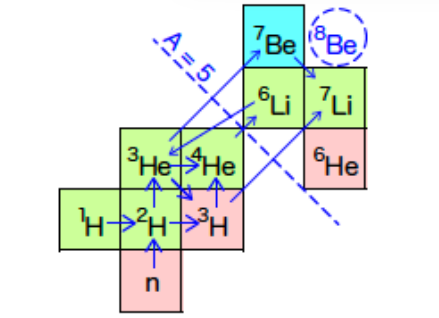
\includegraphics[width=8cm]{./assets/nuclear.png}
    \caption{}
    \label{fig:2level}
  \end{center}
\end{figure}

\begin{table}[hbtp]
  \centering
  \begin{tabular}{|c|c|c|c|}
    \hline
    宇宙開闢からの時間        & 温度            & 反応式                                                & 終了後                                \\
    \hline \hline
    $10^{-6}$ \si{s} & 1 \si{GeV}    & quauk $\to p, n$                                   &                                    \\
    -1 \si{s}        & 0.7 \si{MeV}  & $n + \nu_e\leftrightarrow p + e^-$                 & $p:n\approx 7:1$ に固定               \\
                     &               & $p + \overline{\nu}_e \leftrightarrow n + e^+$     &                                    \\
    0.1 \si{s}       & 0.1 \si{MeV}  & $n + p \leftrightarrow d + \gamma (2.23 \si{MeV})$ & 平衡状態終了後 $d$ 増加                     \\
    $10^3$ \si{s}    & 0.03 \si{MeV} & $\ce{^4He} + d \to \ce{^6Li} + \gamma$             & 中性子捕獲が進み $n$ 枯渇, 温度低下              \\
                     &               & $\ce{^4He} + t\to \ce{^7Li} + \gamma$              &                                    \\
                     &               & $\ce{^4He} + \ce{^3He}\to \ce{^7Be} + \gamma$      & \ce{^7Be},\ce{^6Li},\ce{^7Li} 少量生成 \\
    その後              &               & $\ce{^7Be} + e^-\to \ce{^7Li} + \nu_e$             &                                    \\
                     &               & $t\to\ce{^3He} + e^- + \nu_e$                      &                                    \\
    \hline
  \end{tabular}
  \caption{Big Bang Nucleosynthesis (BBN)}
  \label{table:big bang nucleosynthesis}
\end{table}

\ce{^7Li} は 3 倍違う: \ce{^7Li} 問題

\begin{align}
  \ce{4^1H \to ^4He + 2e^+ + 2\nu}
\end{align}
赤色巨星の一種 AGB 星 (Asymptotic Giant Branch)  sプロセス

r-プロセス (Rapid プロセス)
中性子捕獲の遷移確率 >> ベータ崩壊の遷移確率
中性子星合体または超新星爆発(高密度,高温)
中性子捕獲と光吸収崩壊が平衡化する。

ベータ崩壊の寿命と
\begin{align}
  \ce{^68Ni} + n & \to \ce{^69Ni} + \gamma                                             \\
  \ce{^69Ni} + n & \to \ce{^70Ni} + \gamma                                             \\
  \ce{^70Ni} + n & \to \ce{^71Ni} + \gamma                                             \\
                 & \vdots                                                              \\
  \ce{^77Ni} + n & \to \ce{^78Ni} + \gamma                                             \\
  \ce{^78Ni} + n & \leftrightarrow \ce{^79Ni} + \gamma \qquad (\textrm{Waiting point})
\end{align}
太陽光のスペクトル+太陽モデル

\begin{table}[hbtp]
  \centering
  \begin{tabular}{|c|c|c|c|c|}
    \hline
    段階     & 反応式                                                     & 時間スケール           & 温度 ($T\times 10^9$ \si{K}) & 密度 (\si{g/cm^3})            \\
    \hline \hline
    水素燃焼   & $4\ce{H} \to \ce{^4He} + \gamma$                        & $7\times 10^6$ y & 0.06                       & 5                           \\
    ヘリウム燃焼 & $3\ce{^4He} \to 3\alpha \to \ce{^12C} + \gamma$ (ホイル状態) & $5\times 10^5$ y & 0.23                       & $7\times 10^2$              \\
    炭素燃焼   & $\ce{^12C} + \ce{^4He} \to \ce{^16O} + \gamma$          & 600 y            & 0.93                       & $2\times 10^5$              \\
    ネオン燃焼  & $\ce{^20Ne} + \gamma \to \ce{^16O} + \ce{^4He}$         & 1 y              & 1.7                        & $4\times 10^6$              \\
    酸素燃焼   & $\ce{^16O} + \ce{^16O}\to\ce{^28Si} + \ce{^4He}$        & 6 months         & 2.3                        & $1\times 10^7$              \\
    Si 燃焼  & $\ce{^28Si} + \ce{^4He}\to\ce{^32S}$                    & 1 d              & 4.1                        & $3\times 10^7$              \\
    コア崩壊   &                                                         & seconds          & 8.1                        & $3\times 10^9$              \\
    コア跳ね返り &                                                         & milliseconds     & 34.8                       & $3\times 10^{14}\sim\rho_0$ \\
    爆発的燃焼  &                                                         & 0.1-10 s         & 1.2-7.0                    &                             \\
    \hline
  \end{tabular}
  \caption{$25M_{sun}$ の星の時系列}
  \label{table:star}
\end{table}

\section{ハドロン物理学}
中性子数が多いからアイソスピン正
電荷との関係によるから陽子が正
\begin{align}
  Q
\end{align}




\end{document}
